\begin{enumerate}
  \item If $\tan\brak{\frac{x+y}{x-y}}=k$, then $\frac{dy}{dx}$ is equal to
    \begin{enumerate}
        \item $ \frac{-y}{x} $
        \item $  \frac{y}{x} $ 
        \item $ \sec^2\brak{\frac{y}{x}}$ 
        \item $ -\sec^2\brak{\frac{y}{x}} $  
    \end{enumerate}
    \item \textbf{Assertion(A):} Maximum value of $(\cos^{-1} x)^2$ is $\pi^2$.\\
    \textbf{Reason(R):} Range of the principal value branch of $\cos^{-1}x$ is $\sbrak{\frac{-\pi}{2},\frac{\pi}{2}}$
    \item \begin{enumerate}
                \item If $ y= \sqrt{ax + b} $, then prove that $y\brak{\frac{d^2y}{dx^2}} + \brak{\frac{dy}{dx}}^2 = 0$
              \item If $f(x) = 
              \begin{cases}
              ax + b & \quad  0 \le x \leq 1\\
              2x^2 - x & \quad 1 \le x \le 2
              \end{cases}$ is a differentiable function in (0, 2), then find the values of a and b.
        \end{enumerate}
\item If the circumference of the circle is increasing at a constant rate , prove that the rate of change of area of the circle is directly proportional to its radius.
 \item Engine displacement is the measure of the cylinder volume swept by all pistons of a piston engine. The piston moves inside the cylinder bore.
		\figref{fig:fig1}
\begin{figure}[h!]
		\centering
		  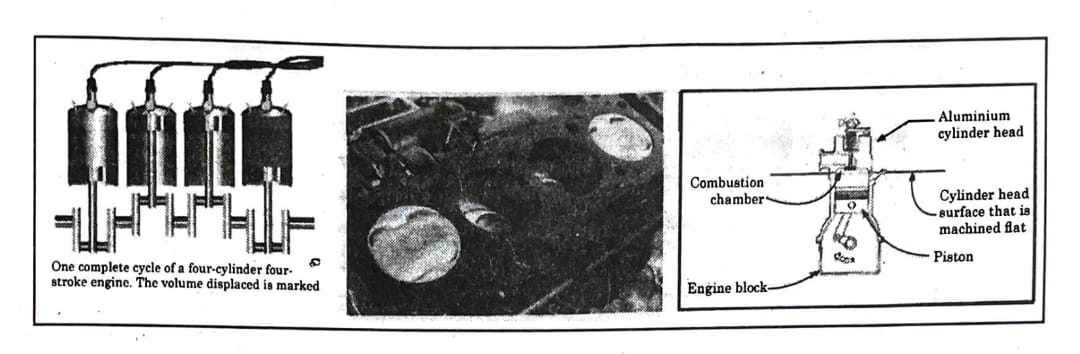
\includegraphics[height=7cm,width=12cm]{./figs/q1.png}
\caption{cylinder bore}
\label{fig:fig1}
\end{figure}
The cylinder bore in the form of circular cylinder open at the top is to be made from a metal sheet of area $75\pi cm^2$.\\Based on the above information, answer the following questions:
		  \begin{enumerate}
			  \item If the radius of cylinder is r cm and height is h cm, then write the volume V of cylinder in terms of radius r.
			  \item Find $\frac{dV}{dr}.$
			  \item \begin{enumerate}

					  \item Find the radius  of cylinder when its volume is maximum.
					  \item For maximum volume,$ h \ge r.$ State true or false and justify.
			  \end{enumerate}
		  \end{enumerate}
	  \item The use of electric vehicles will curb air pollution in the long run.
\figref{fig:Fig2}
		\begin{figure}[h!]
		\centering
		  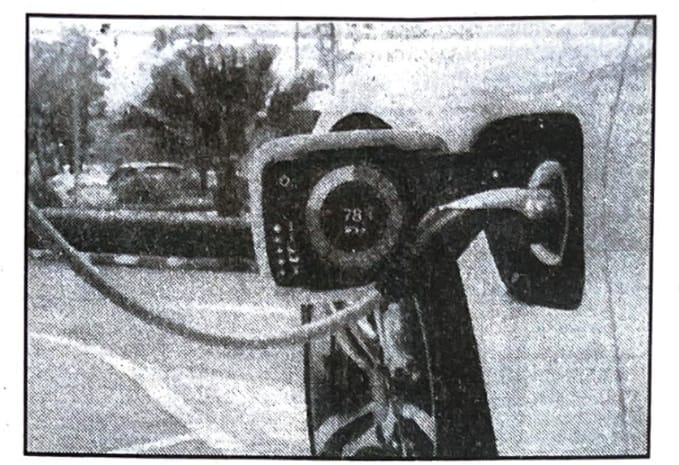
\includegraphics[height=7cm,width=11cm]{./figs/q3.png}
\caption{car}
\end{figure}
		  The use of electric vehicles is increasing every year and estimated electric vehicles in use at any time t is given by the function V:\\
	 \quad $V(t) = \frac{1}{5}t^3 - \frac{5}{2}t^2 + 25t - 2 $\\where t represents the time and t = 1, 2, 3.... corresponds to year 2001,2002, 2003,.....respectively.\\Based on the above information, answer the following questions:
		  \begin{enumerate}
			  \item Can the above function be used to estimate number of vehicles in the year 2000 ? Justify.
			  \item Prove that the function V(t) is an increasing function.
		  \end{enumerate}

 \end{enumerate}
